\documentclass{article}%

\usepackage{amsmath}%
\usepackage{amsfonts}%
\usepackage{amssymb}%
\usepackage{graphicx}
\usepackage[english,greek]{babel}
\usepackage[utf8x]{inputenc}
\usepackage{listings}
\usepackage{lipsum}
\begin{document}


\selectlanguage{greek}

\title{Δίκτυα Επικοινωνιών\\6η εργαστηριακή άσκηση\\  \indent \\
\textbf{Επίδοση Τοπικών ∆ικτύων \textlatin{IEEE 802.3}} }
\author{Γεώργιος Δασούλας\\Α.Μ: 03112010 \\ 6ο Εξάμηνο 2014-2015  }
\date{\today}
\maketitle

Σε αυτή την άσκηση θα μελετηθεί η επίδοση του $MAC$ πρωτοκόλλου $IEEE$ $802.3$. Για το σκοπό αυτό θα
μετρηθεί το πλήθος των πακέτων και η ποσότητα των δεδομένων που μεταδόθηκαν επιτυχώς κατά τη
διάρκεια της προσομοίωσης, καθώς και η μέση καθυστέρηση των πακέτων. Από αυτά τα δεδομένα θα
γίνει υπολογισμός της χρησιμοποίησης του καναλιού και σύγκριση με τα θεωρητικά αναμενόμενα
αποτελέσματα.\\


\textbf{\large{\underline{Μελέτη απόδοσης τοπικού δικτύου ΙΕΕΕ 802.3}}}\\ 
Με βάση την προσομοίωση που εκτελέσαμε θα επαληθεύσουμε κατά πόσον ισχύει ή όχι η εξίσωση:
$\displaystyle{\eta= \frac{P}{P+2*\tau*e}}$.
Όπου:
\begin{itemize}
\item $\eta$ είναι η απόδοση του διαύλου (πραγματικός ρυθμός μεταφοράς δεδομένων / ονομαστικό
ρυθμό μετάδοσης ζεύξης) 
\item $P$ είναι ο χρόνος μετάδοσης κάθε πλαισίου (Μήκος πλαισίου σε bit / ονομαστικό ρυθμό
μετάδοσης ζεύξης)
\item $\tau$ είναι η μέγιστη επιτρεπόμενη καθυστέρηση διάδοσης πάνω στο καλώδιο, την οποία
μπορείτε να θεωρήσετε ίση με \textlatin{25,6 $\mu$ s}.
\item $e$ = 2,718281828
\end{itemize}

Για την επαλήθευση της θεωρητικής τιμής θα εκτελέσουμε μια σειρά προσομοιώσεων, η  οποία πραγματοποιείται με μεταβαλλόμενο μέγεθος πακέτου από \textlatin{64 Byte} (ελάχιστο μέγεθος πλαισίου) μέχρι \textlatin{1500 Byte} (μέγιστο μέγεθος πλαισίου). Πραγματοποιήσαμε 10 προσομοιώσεις. Για την πειραματική τιμή χρησιμοποίησαμε τον τύπο:
$\eta = \frac{numberpackets*packetsize*8}{(endtime-starttime)*10000000}$.
\newpage 
Μετά τον τροποποιημένο κώδικα ακολουθούν οι καμπύλες :
Για τη χάραξη της γραφικής με το χρόνο τελευταίας επιτυχημένης λήψης τροποποίησαμε τον κώδικα $awk$ ώς εξής :\\
\selectlanguage{english}
\begin{verbatim}
BEGIN {
 sum_delay = 0;
 bufferspace = 100000;
 total_pkts_sent = 0;
 total_pkts_recv = 0;
 lastpackt_recv=0;
 total_pkts_dropped = 0;

 if (sprintf(sqrt(2)) ~ /,/) dmfix = 1;
}

{
 if (dmfix) sub(/\./, ",", $0);
}
/^h/&&/cbr/ {
 total_pkts_sent++;
}
/^d/&&/cbr/ {
 total_pkts_dropped++;
} 
8
/^-/&&/cbr/ {
 sendtimes[$12%bufferspace] = $2;
}
/^r/&&/cbr/ {
 pkts_recv++;
 sum_delay += $2 - sendtimes[$12%bufferspace]
 lastpackt_recv=$2;
}
END {

 printf("Last packet received \t: %f sec\n", 1.0*lastpackt_recv);
 } 
\end{verbatim}
\selectlanguage{greek}


\begin{figure}[htbp]
	\centering
		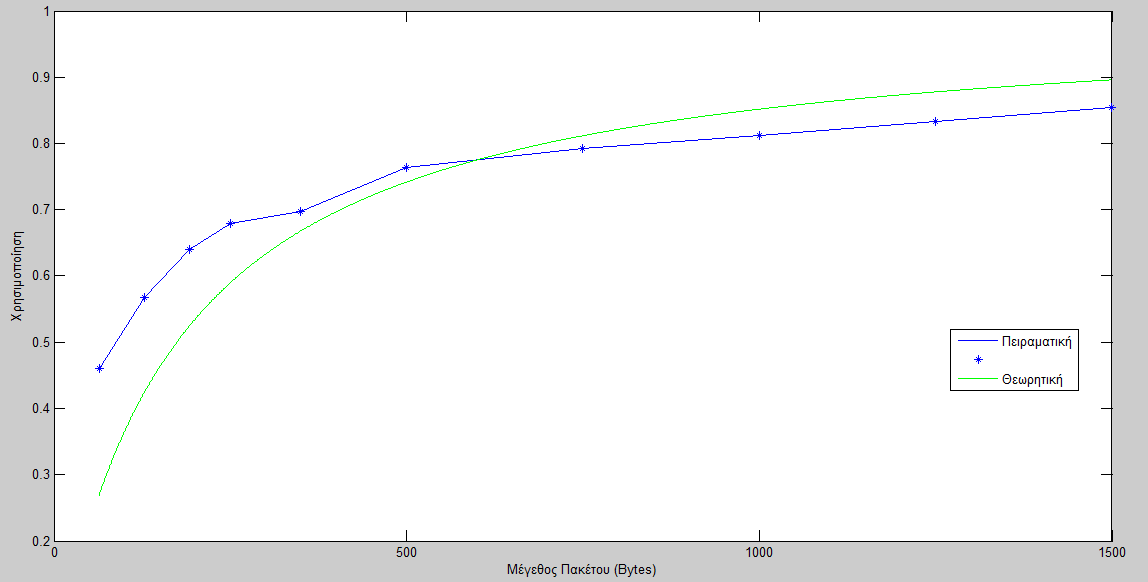
\includegraphics[width=0.7\textwidth]{1.png}
	\caption{Χρησιμοποίηση καναλιού}
	\label{fig:1}
\end{figure}

\begin{figure}[htbp]
	\centering
		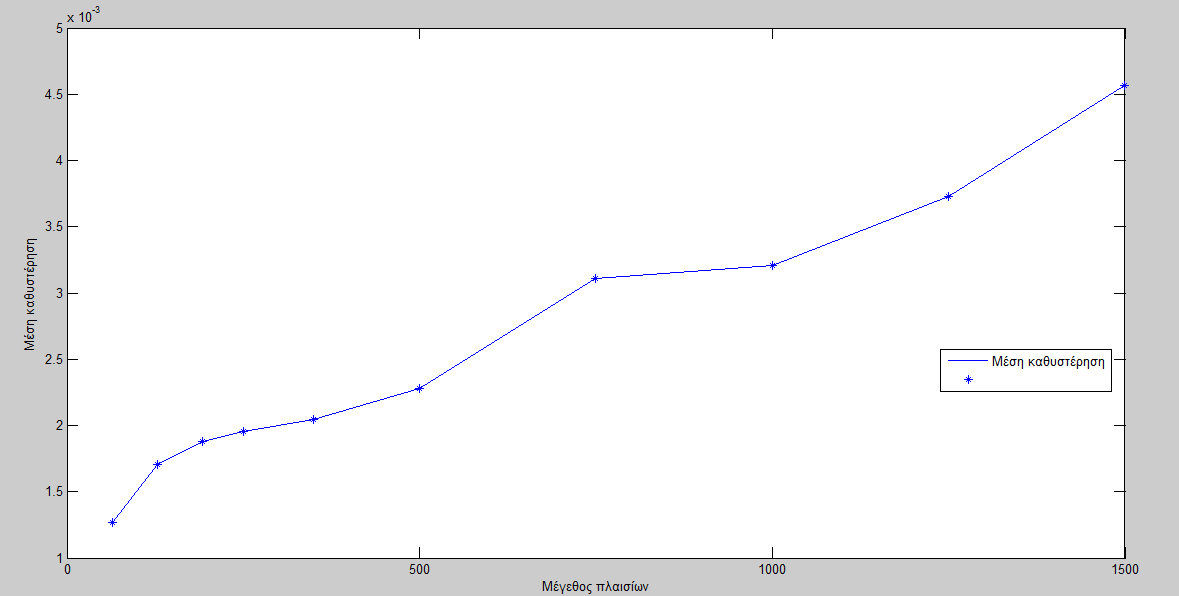
\includegraphics[width=0.7\textwidth]{2.png}
	\caption{Μέση καθυστέρηση}
	\label{fig:2}
\end{figure}

\begin{figure}[htbp]
	\centering
		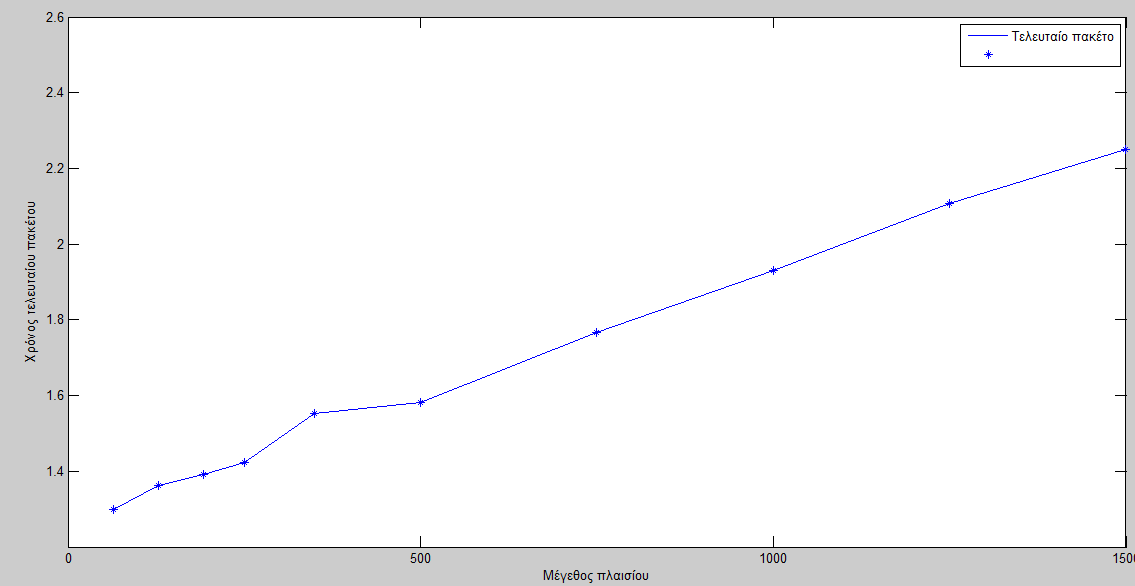
\includegraphics[width=0.7\textwidth]{3.png}
	\caption{Τελευταία λήψη}
	\label{fig:3}
	\end{figure}
	
	\newpage
	
Από τις παραπάνω γραφικές βλέπουμε πως είναι προτιμότερο να χρησιμοποιούμε μεγάλα πλαίσια. Αυτό προκύπτει τόσο από την πειραματική καμπύλη που βλέπουμε να πλησιάζει προς το 1, όσο και από τη θεωρητική γραφική παράσταση, καθώς όσο το μέγεθος του πλαισίου μεγαλώνει , τόσο η χρησιμοποιήση του καναλιού προσεγγίζει το 1. Βέβαια , παρατηρώντας και τις τρεις γραφικές , συμπεραίνουμε πως όσο μεγαλώνουμε το πλαίσιο, τόσο αυξάνεται η μέση καθυστέρηση και ο χρόνος της τελευταίας επιτυχημένης λήψης. Γι' αυτό, αποσκοπώντας στη μεγαλύτερη χρησιμοποίηση του καναλιού έχουμε κάποιο κόστος στην καθυστέρηση και  χρόνο λήψης.


\textbf{\large{Επίδραση αριθμού σταθμών}}\\

Με την κατάλληλη τροποποίηση του $awk$ και του $tcl$ αρχείου προέκυψαν τα παρακάτω:
\begin{table}[h]
\begin{tabular}{|l|l|l|l|}
\hline
Χρησιμοποίηση & Καθυστέρηση & Ποσοστό απορριφθέντων & Πλήθος σταθμών \\ \hline
0.781441      & 0.002163    & 55.5783               & 5              \\ \hline
0.790721      & 0.002034    & 54.0491               & 10             \\ \hline
0.799827      & 0.002781    & 48.4032               & 15             \\ \hline
0.816552      & 0.003562    & 44.1465               & 20             \\ \hline
\end{tabular}
\end{table}
\begin{figure}[htbp]
	\centering
		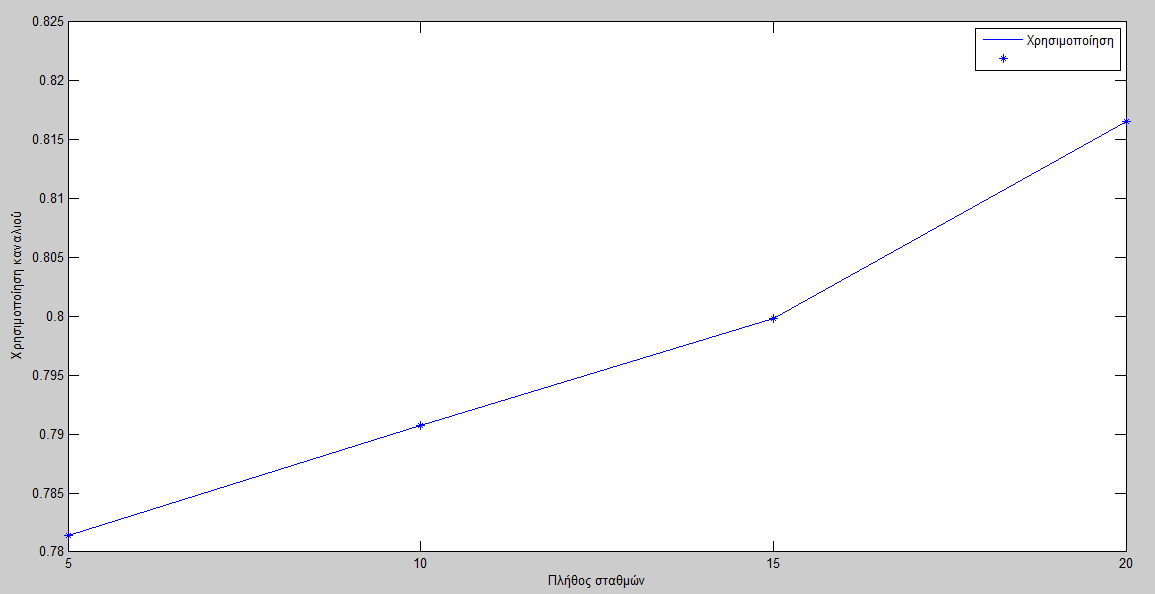
\includegraphics[width=0.7\textwidth]{4.png}
	\caption{Χρησιμοποίηση καναλιού}
	\label{fig:4}
\end{figure}

\begin{figure}[htbp]
	\centering
		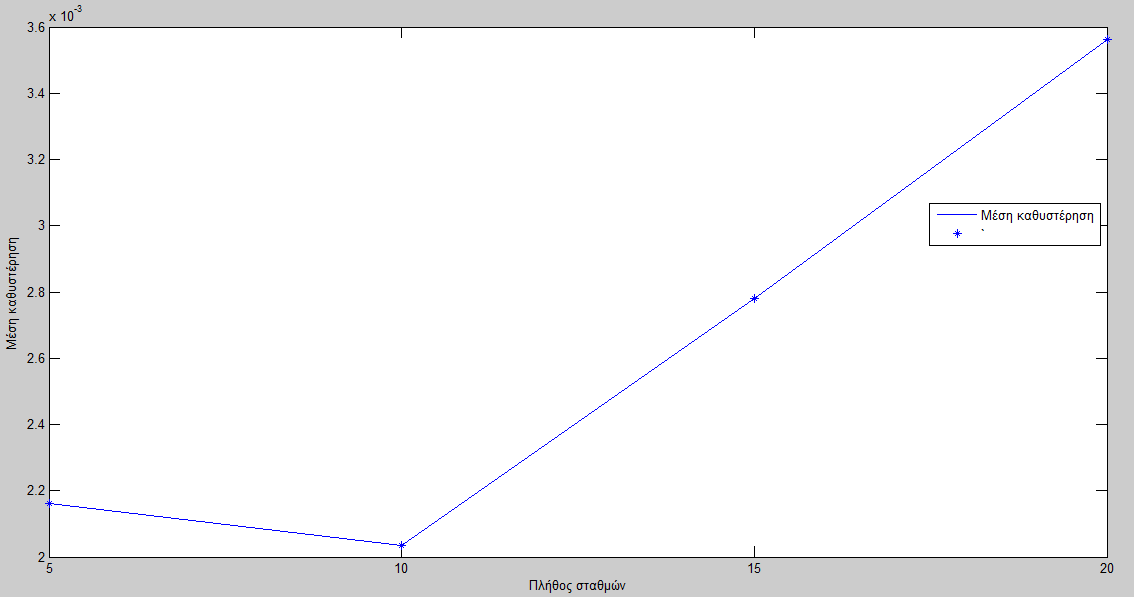
\includegraphics[width=0.7\textwidth]{5.png}
	\caption{Μέση καθυστέρηση}
	\label{fig:5}
\end{figure}


\begin{figure}[htbp]
	\centering
		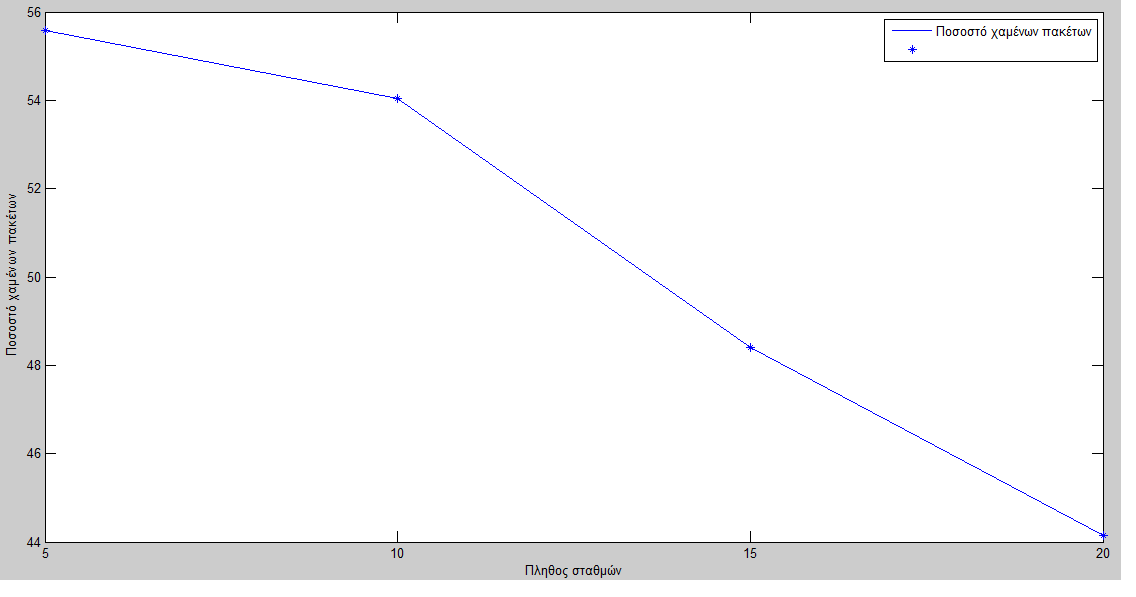
\includegraphics[width=0.7\textwidth]{6.png}
	\caption{Ποσοστό χαμένων πακέτων}
	\label{fig:6}
\end{figure}
\newpage
(β) Καταρχάς , παρατηρούμε πως η χρησιμοποίηση του καναλιού αυξάνεται , όχι αισθητά, με την αύξηση των σταθμών, κάτι το οποίο οφείλεται στο ότι οι περισσότεροι κόμβοι διευκολύνουν τη μεταφορά δεδομένων. Επίσης, με την αύξηση των σταθμών έχουμε και μεγαλύτερη καθυστέρηση , κάτι το οποίο και πάλι οφείλεται στο ότι αυξάνεται η τοπολογία μας και στο ότι υπάρχουν περισσότεροι κόμβοι που πρέπει να δώσουν και να πάρουν πακέτα δεδομένων. Τέλος , τα απορριφθέντα πακέτα μειώνονται , κάτι το οποίο οφείλεται και πάλι στην αύξηση των κόμβων , μιας και διευκολύνεται έτσι η μετάδοση των δεδομένων χωρίς υπερχείλιση πληροφοριών.
\end{document}